% Framework architecture diagram — methodology-first labels
\documentclass[tikz,border=6pt]{standalone}
\usepackage[T1]{fontenc}
\usepackage{lmodern}
\usetikzlibrary{arrows.meta,positioning,fit,backgrounds,calc}

\begin{document}
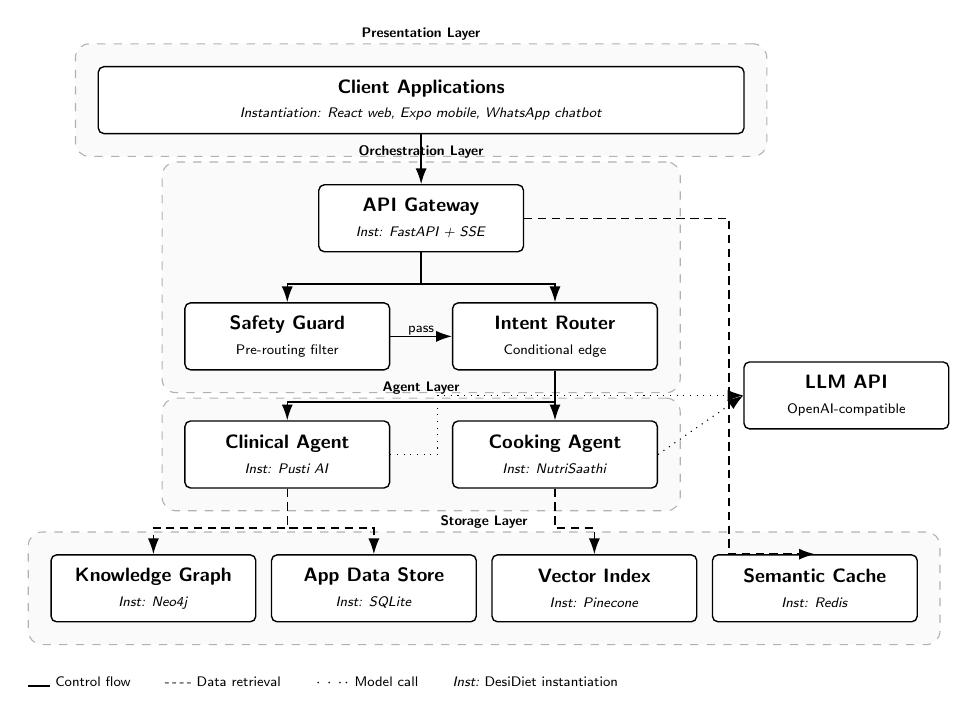
\begin{tikzpicture}[
  font=\sffamily\scriptsize,
  every node/.style={inner sep=0pt},
  box/.style={
    draw=black, fill=white, rounded corners=2pt,
    minimum width=2.6cm, minimum height=0.85cm,
    align=center, line width=0.5pt,
  },
  grp/.style={draw=gray!60, rounded corners=5pt, inner sep=8pt,
    line width=0.4pt, fill=gray!4, dashed},
  glbl/.style={font=\sffamily\tiny\bfseries, text=black},
  inst/.style={font=\sffamily\tiny, text=gray!70!black},
  flow/.style={-{Latex[length=2mm, width=1.4mm]}, line width=0.5pt, draw=black},
  data/.style={-{Latex[length=2mm, width=1.4mm]}, line width=0.5pt, draw=black, densely dashed},
  modl/.style={-{Latex[length=2mm, width=1.4mm]}, line width=0.4pt, draw=black, dotted},
]

% ===== ROW 1: CLIENT APPLICATIONS (y=0) =====
\node[box, minimum width=8.2cm] (clients) at (3.4, 0) {%
  \textbf{Client Applications}\\[1pt]
  \tiny\textit{Instantiation: React web, Expo mobile, WhatsApp chatbot}};

% ===== ROW 2: BACKEND (y=-1.5) =====
\node[box] (api) at (3.4, -1.5) {\textbf{API Gateway}\\[1pt]\tiny\textit{Inst: FastAPI + SSE}};

% ===== ROW 3: GUARD + ROUTER (y=-3.0) =====
\node[box] (guard)  at (1.7, -3.0) {\textbf{Safety Guard}\\[1pt]\tiny Pre-routing filter};
\node[box] (router) at (5.1, -3.0) {\textbf{Intent Router}\\[1pt]\tiny Conditional edge};

% ===== ROW 4: AGENTS (y=-4.5) =====
\node[box] (clinical) at (1.7, -4.5) {\textbf{Clinical Agent}\\[1pt]\tiny\textit{Inst: Pusti AI}};
\node[box] (cooking) at (5.1, -4.5) {\textbf{Cooking Agent}\\[1pt]\tiny\textit{Inst: NutriSaathi}};

% ===== ROW 5: DATA STORES (y=-6.2) =====
\node[box] (kg)    at (0, -6.2) {\textbf{Knowledge Graph}\\[1pt]\tiny\textit{Inst: Neo4j}};
\node[box] (app)   at (2.8, -6.2) {\textbf{App Data Store}\\[1pt]\tiny\textit{Inst: SQLite}};
\node[box] (vec)   at (5.6, -6.2) {\textbf{Vector Index}\\[1pt]\tiny\textit{Inst: Pinecone}};
\node[box] (cache) at (8.4, -6.2) {\textbf{Semantic Cache}\\[1pt]\tiny\textit{Inst: Redis}};

% ===== EXTERNAL: LLM =====
\node[box] (llm) at (8.8, -3.75) {\textbf{LLM API}\\[1pt]\tiny OpenAI-compatible};

% ===== GROUP BACKGROUNDS =====
\begin{scope}[on background layer]
  \node[grp, fit=(clients)] (g1) {};
  \node[glbl, above=1pt of g1.north] {\textsc{Presentation Layer}};

  \node[grp, fit=(api)(guard)(router)] (g2) {};
  \node[glbl, above=1pt of g2.north] {\textsc{Orchestration Layer}};

  \node[grp, fit=(clinical)(cooking)] (g3) {};
  \node[glbl, above=1pt of g3.north] {\textsc{Agent Layer}};

  \node[grp, fit=(kg)(app)(vec)(cache)] (g4) {};
  \node[glbl, above=1pt of g4.north] {\textsc{Storage Layer}};
\end{scope}

% ===== ARROWS: Client -> Backend =====
\draw[flow] (clients.south) -- (api.north);

% ===== ARROWS: Backend -> Guard -> Router =====
\draw[flow] (api.south) -- ++(0,-0.4) -| (guard.north);
\draw[flow] (api.south) -- ++(0,-0.4) -| (router.north);
\draw[flow] (guard.east) -- node[above, font=\tiny\sffamily]{pass} (router.west);

% ===== ARROWS: Router -> Agents =====
\draw[flow] (router.south) -- ++(0,-0.4) -| (clinical.north);
\draw[flow] (router.south) -- ++(0,-0.4) -| (cooking.north);

% ===== ARROWS: Agents -> Data Stores =====
\draw[data] (clinical.south) -- ++(0,-0.5) -| (kg.north);
\draw[data] (clinical.south) -- ++(0,-0.5) -| (app.north);
\draw[data] (cooking.south) -- ++(0,-0.5) -| (vec.north);
\draw[data] (api.east) -- ++(2.6,0) |- (cache.north);

% ===== ARROWS: Agents -> LLM =====
\draw[modl] (clinical.east) -- ++(0.6,0) |- (llm.west);
\draw[modl] (cooking.east) -- (llm.west);

% ===== LEGEND =====
\node[anchor=north west, font=\sffamily\tiny, text=black] at ($(g4.south west)+(0,-0.4)$) {%
  {\rule{8pt}{0.8pt}}~Control flow
  \qquad {-\,-\,-\,-}~Data retrieval
  \qquad {$\cdot\cdot\cdot\cdot$}~Model call
  \qquad \textit{Inst:}~DesiDiet instantiation
};

\end{tikzpicture}
\end{document}
